%beamer

% TODO:
% - VL-Folien einarbeiten
% - Weniger f_* etc. Theorie, mehr Aufgaben zwischendrin und zu Akzeptoren
% - Bessere Hinleitung zu Akzeptoren

% Comment/uncomment this line to toggle handout mode
%\newcommand{\handout}{}

%% Beamer-Klasse im korrekten Modus
\ifdefined \handout
\documentclass[handout]{beamer} % Handout mode
\else
\documentclass{beamer}
\fi

%% UTF-8-Encoding
\usepackage[utf8]{inputenc}

% % \bigtimes abgeschrieben von http://tex.stackexchange.com/questions/14386/importing-a-single-symbol-from-a-different-font
% \DeclareFontFamily{U}{mathx}{\hyphenchar\font45}
% \DeclareFontShape{U}{mathx}{m}{n}{
%       <5> <6> <7> <8> <9> <10> gen * mathx
%       <10.95> mathx10 <12> <14.4> <17.28> <20.74> <24.88> mathx12
%       }{}
% \DeclareSymbolFont{mathx}{U}{mathx}{m}{n}
% \DeclareMathSymbol{\bigtimes}{\mathop}{mathx}{161}

\RequirePackage{xcolor}

\def\9{\square}
%\def\9{\blank}

% f"ur Aussagenlogik
\colorlet{alcolor}{blue}
\RequirePackage{tikz}
\usetikzlibrary{arrows.meta}
\newcommand{\alimpl}{\mathrel{\tikz[x={(0.1ex,0ex)},y={(0ex,0.1ex)},>={Classical TikZ Rightarrow[]}]{\draw[alcolor,->,line width=0.7pt,line cap=round] (0,0) -- (15,0);\path (0,-6);}}}
\newcommand{\aleqv}{\mathrel{\tikz[x={(0.1ex,0ex)},y={(0ex,0.1ex)},>={Classical TikZ Rightarrow[]}]{\draw[alcolor,<->,line width=0.7pt,line cap=round] (0,0) -- (18,0);\path (0,-6);}}}
\newcommand{\aland}{\mathbin{\raisebox{-0.6pt}{\rotatebox{90}{\texttt{\color{alcolor}\char62}}}}}
\newcommand{\alor}{\mathbin{\raisebox{-0.8pt}{\rotatebox{90}{\texttt{\color{alcolor}\char60}}}}}
%\newcommand{\ali}[1]{_{\mathtt{\color{alcolor}#1}}}
\newcommand{\alv}[1]{\mathtt{\color{alcolor}#1}}
\newcommand{\alnot}{\mathop{\tikz[x={(0.1ex,0ex)},y={(0ex,0.1ex)}]{\draw[alcolor,line width=0.7pt,line cap=round,line join=round] (0,0) -- (10,0) -- (10,-4);\path (0,-8) ;}}}
\newcommand{\alP}{\alv{P}} %ali{#1}}
%\newcommand{\alka}{\negthinspace\hbox{\texttt{\color{alcolor}(}}}
\newcommand{\alka}{\negthinspace\text{\texttt{\color{alcolor}(}}}
%\newcommand{\alkz}{\texttt{\color{alcolor})}}\negthinspace}
\newcommand{\alkz}{\text{\texttt{\color{alcolor})}}\negthinspace}
\newcommand{\AAL}{A_{AL}}
\newcommand{\LAL}{\hbox{\textit{For}}_{AL}}
\newcommand{\AxAL}{\hbox{\textit{Ax}}_{AL}}
\newcommand{\AxEq}{\hbox{\textit{Ax}}_{Eq}}
\newcommand{\AxPL}{\hbox{\textit{Ax}}_{PL}}
\newcommand{\AALV}{\hbox{\textit{Var}}_{AL}}
\newcommand{\MP}{\hbox{\textit{MP}}}
\newcommand{\GEN}{\hbox{\textit{GEN}}}
\newcommand{\W}{\ensuremath{\hbox{\textbf{w}}}\xspace}
\newcommand{\F}{\ensuremath{\hbox{\textbf{f}}}\xspace}
\newcommand{\WF}{\ensuremath{\{\W,\F\}}\xspace}
\newcommand{\val}{\hbox{\textit{val}}}
\newcommand{\valDIb}{\val_{D,I,\beta}}

\newcommand*{\from}{\colon}

% die nachfolgenden Sachen angepasst an cmtt
\newlength{\ttquantwd}
\setlength{\ttquantwd}{1ex}
\newlength{\ttquantht}
\setlength{\ttquantht}{6.75pt}
\def\plall{%
  \tikz[line width=0.67pt,line cap=round,line join=round,baseline=(B),alcolor] {
    \draw (-0.5\ttquantwd,\ttquantht) -- node[coordinate,pos=0.4] (lll){} (-0.25pt,-0.0pt) -- (0.25pt,-0.0pt) -- node[coordinate,pos=0.6] (rrr){} (0.5\ttquantwd,\ttquantht);
    \draw (lll) -- (rrr);
    \coordinate (B) at (0,-0.35pt);
  }%
}
\def\plexist{%
  \tikz[line width=0.67pt,line cap=round,line join=round,baseline=(B),alcolor] {
    \draw (-0.9\ttquantwd,\ttquantht) -- (0,\ttquantht) -- node[coordinate,pos=0.5] (mmm){} (0,0) --  (-0.9\ttquantwd,0);
    \draw (mmm) -- ++(-0.75\ttquantwd,0);
    \coordinate (B) at (0,-0.35pt);
  }\ensuremath{\,}%
}
\let\plexists=\plexist
\newcommand{\NT}[1]{\ensuremath{\langle\mathrm{#1} \rangle}}

\newcommand{\CPL}{\text{\itshape Const}_{PL}}
\newcommand{\FPL}{\text{\itshape Fun}_{PL}}
\newcommand{\RPL}{\text{\itshape Rel}_{PL}}
\newcommand{\VPL}{\text{\itshape Var}_{PL}}
\newcommand{\ATer}{A_{\text{\itshape Ter}}}
\newcommand{\ARel}{A_{\text{\itshape Rel}}}
\newcommand{\AFor}{A_{\text{\itshape For}}}
\newcommand{\LTer}{L_{\text{\itshape Ter}}}
\newcommand{\LRel}{L_{\text{\itshape Rel}}}
\newcommand{\LFor}{L_{\text{\itshape For}}}
\newcommand{\NTer}{N_{\text{\itshape Ter}}}
\newcommand{\NRel}{N_{\text{\itshape Rel}}}
\newcommand{\NFor}{N_{\text{\itshape For}}}
\newcommand{\PTer}{P_{\text{\itshape Ter}}}
\newcommand{\PRel}{P_{\text{\itshape Rel}}}
\newcommand{\PFor}{P_{\text{\itshape For}}}

\newcommand{\plka}{\alka}
\newcommand{\plkz}{\alkz}
%\newcommand{\plka}{\plfoo{(}}
%\newcommand{\plkz}{\plfoo{)}}
\newcommand{\plcomma}{\hbox{\texttt{\color{alcolor},}}}
\newcommand{\pleq}{{\color{alcolor}\,\dot=\,}}

% MODIFIED (DJ)
% previously: \newcommand{\plfoo}[1]{\mathtt{\color{alcolor}#1}}
\newcommand{\plfoo}[1]{\texttt{\color{alcolor}#1}}

\newcommand{\plc}{\plfoo{c}}
\newcommand{\pld}{\plfoo{d}}
\newcommand{\plf}{\plfoo{f}}
\newcommand{\plg}{\plfoo{g}}
\newcommand{\plh}{\plfoo{h}}
\newcommand{\plx}{\plfoo{x}}
\newcommand{\ply}{\plfoo{y}}
\newcommand{\plz}{\plfoo{z}}
\newcommand{\plR}{\plfoo{R}}
\newcommand{\plS}{\plfoo{S}}

\newcommand{\bv}{\mathrm{bv}}
\newcommand{\fv}{\mathrm{fv}}

%\newcommand{\AxAL}{\hbox{\textit{Ax}}_{AL}}
%\newcommand{\AALV}{\hbox{\textit{Var}}_{AL}}

%\renewcommand{\#}[1]{\literal{#1}}
\newcommand{\A}{\mathcal{A}}
\newcommand{\Adr}{\text{Adr}}
\newcommand{\ar}{\mathrm{ar}}
\newcommand{\ascii}[1]{\literal{\char#1}}
%\newcommand{\assert}[1]{\text{/\!\!/\ } #1}
\newcommand{\assert}[1]{\colorbox{black!7!white}{\ensuremath{\{\;#1\;\}}}}
\newcommand{\Assert}[1]{$\langle$\textit{#1}$\rangle$}
\newcommand{\B}{\mathcal{B}}
\newcommand{\bfmod}{\mathbin{\kw{ mod }}}
\newcommand{\bb}{{\text{bb}}}
\def\bottom{\hbox{\small$\pmb{\bot}$}}
\newcommand{\card}[1]{|#1|}
%\newcommand{\cod}{\mathop{\text{cod}}}  % ist in thwmathabbrevs
\newcommand{\Conf}{\mathcal{C}}
\newcommand{\define}[1]{\emph{#1}}
%\renewcommand{\dh}{d.\,h.\@\xspace}
%\newcommand{\Dh}{D.\,h.\@\xspace}
%\newcommand{\engl}[1]{engl.\xspace\emph{#1}}
\newcommand{\eps}{\varepsilon}
%\newcommand{\evtl}{evtl.\@\xspace}
\newcommand{\fbin}{\text{bin}}
\newcommand{\finv}{\text{inv}}
\newcommand{\fnum}{\text{num}}
\newcommand{\fNum}{{\text{Num}}}
\newcommand{\frepr}{\text{repr}}
\newcommand{\fRepr}{\text{Repr}}
\newcommand{\fZkpl}{\text{Zkpl}}
\newcommand{\fLen}{\text{Len}}
\newcommand{\fsem}{\text{sem}}
\providecommand{\fspace}{\mathord{\text{space}}}
\providecommand{\fSpace}{\mathord{\text{Space}}}
\providecommand{\ftime}{\mathord{\text{time}}}
\providecommand{\fTime}{\mathord{\text{Time}}}
\newcommand{\fTrans}{\text{Trans}}
\newcommand{\fVal}{\text{Val}}

% MODIFIED (DJ)
\newcommand{\Val}{\text{Val}}

%\def\G{\mathbb{Z}}
\newcommand{\HT}[1]{\normalfont\textsc{HT-#1}}
\newcommand{\htr}[3]{\{#1\}\;#2\; \{#3\}}
\newcommand{\Id}{\text{I}}
%\newcommand{\ie}{i.\,e.\@\xspace}
\newcommand{\instr}[2]{\texttt{#1}\ \textit{#2}}
\newcommand{\Instr}[2]{\texttt{#1}\ \textrm{#2}}
\newcommand{\instrr}[3]{\texttt{#1}\ \textit{#2}\texttt{(#3)}}
\newcommand{\Instrr}[3]{\texttt{#1}\ \textrm{#2}\texttt{(#3)}}

% MODIFIED (DJ)
% previously:  \newcommand{\io}{\!\mid\!}
\newcommand{\io}{\ensuremath{\!\mid\!}}

\usepackage{KITcolors}
\newcommand{\literal}[1]{\hbox{\textcolor{blue!95!white}{\textup{\texttt{\scalebox{1.11}{#1}}}}}}
%\newcommand{\literal}[1]{\hbox{\textcolor{KITblue!80!black}{\textup{\texttt{#1}}}}}
\def\kasten#1{\leavevmode\literal{\setlength{\fboxsep}{1pt}\fbox{\vrule  width 0pt height 1.5ex depth 0.5ex #1}}}
\newcommand{\kw}[1]{\ensuremath{\mathbf{#1}}}
\newcommand{\lang}[1]{\ensuremath{\langle#1\rangle}}
%\newcommand{\maw}{m.\,a.\,w.\@\xspace}
%\newcommand{\MaW}{M.\,a.\,w.\@\xspace}
\newcommand{\mdefine}[2][FOOBAR]{\define{#2}\def\foobar{FOOBAR}\def\optarg{#1}\ifx\foobar\optarg\def\optarg{#2}\fi\graffito{\optarg}}
\newcommand{\meins}{\rotatebox[origin=c]{180}{1}}
\newcommand{\Mem}{\text{Mem}}
\newcommand{\memread}{\text{memread}}
\newcommand{\memwrite}{\text{memwrite}}
\providecommand{\meta}[1]{\ensuremath{\langle}\textit{#1}\ensuremath{\rangle}}
%\newcommand{\N}{\mathbb{N}}
\newcommand{\NP}{\mathbf{NP}}
\newcommand{\Nadd}{N_{\text{add}}}
\newcommand{\Nmult}{N_{\text{mult}}}
% MODIFIED (DJ): added \!, mathcal{O}
\newcommand{\Oh}[1]{\mathcal{O}\!\left(#1\right)}
\newcommand{\Om}[1]{\Omega\!\left(#1\right)}
\newcommand{\personname}[1]{\textsc{#1}}
\newcommand{\regname}[1]{\texttt{#1}}
\newcommand{\mima}{\textsc{Mima}\xspace}
\newcommand{\mimax}{\textsc{Mima-X}\xspace}

\def\Pclass{\text{\bfseries P}}
\def\PSPACE{\text{\bfseries PSPACE}}

\newcommand{\SPush}{\text{push}}
\newcommand{\SPop}{\text{pop}}
\newcommand{\SPeek}{\text{peek}}
\newcommand{\STop}{\text{top}}
\newcommand{\STos}{\text{\itshape tos}}
\newcommand{\SBos}{\text{\itshape bos}}

%\newcommand{\R}{\mathbb{R}}
\newcommand{\Rnullplus}{\R_0^{+}}
\newcommand{\Rplus}{\R_{+}}
\newcommand{\resp}{resp.\@\xspace}
\newcommand{\Sem}{\text{Sem}}
\newcommand{\sgn}{\mathop{\text{sgn}}}
\newcommand{\sqbox}{\mathop{\raisebox{-6.2pt}{\hbox{\hbox to 0pt{$^{^{\sqcap}}$\hss}$^{^{\sqcup}}$}}}}
\newcommand{\sqleq}{\sqsubseteq}
\newcommand{\sqgeq}{\sqsupseteq}
% MODIFIED (DJ): added \!
\newcommand{\Th}[1]{\Theta\!\left(#1\right)}
%\newcommand{\usw}{usw.\@\xspace}
\newcommand{\V}[1]{\hbox{\textit{#1}}}
\newcommand{\x}{\times}
\newcommand{\ZK}{\mathbb{K}}
%\newcommand{\Z}{\mathbb{Z}}
\newcommand{\zB}{z.\,B.\@\xspace}
\newcommand{\ZB}{Z.\,B.\@\xspace}
% \newcommand{\bb}{{\text{bb}}}
% \def\##1{\hbox{\textcolor{darkblue}{\texttt{#1}}}}
% \def\A{\mathcal{A}}
% \newcommand{\0}{\#0}
% \newcommand{\1}{\#1}
% \newcommand{\Obj}{\text{Obj}}
% \newcommand{\start}{\mathop{\text{start}}}
% \newcommand{\compactlist}{\addtolength{\itemsep}{-\parskip}}
% \newcommand{\fval}{\text{val}}
% \newcommand{\lang}[1]{\ensuremath{\langle#1\rangle}}
% \newcommand{\io}{\!\mid\!}
% \def\sqbox{\mathop{\raisebox{-6.2pt}{\hbox{\hbox to 0pt{$^{^{\sqcap}}$\hss}$^{^{\sqcup}}$}}}}
% \def\sqleq{\sqsubseteq}
% \def\sqgeq{\sqsupseteq}
\def\Td{T_{\overline{d}}}
% \newcommand{\csym}[1]{\ensuremath{\#{c}_{\#{\hbox{\scriptsize #1}}}}}
% \newcommand{\F}{\ensuremath{\mathcal{F}}}
% \newcommand{\fsym}[2]{\ensuremath{\#{f}^{\#{\hbox{\scriptsize #1}}}_{\#{\hbox{\scriptsize #2}}}}}
% \newcommand{\rsym}[2]{\ensuremath{\#{R}^{\#{\hbox{\scriptsize #1}}}_{\#{\hbox{\scriptsize #2}}}}}
% \newcommand{\xsym}[1]{\ensuremath{\#{x}_{\#{\hbox{\scriptsize #1}}}}}
% \newcommand{\I}{\mathcal{I}}
% ********************************************************************

\usepackage[blue]{../framework/thwregex}
\usepackage{environ}
\usepackage{bm}
\usepackage{calc}
\usepackage{varwidth}
\usepackage{wasysym}
\usepackage{mathtools}

%%%%%%%%%%%%%%%%%%%%%%%%%%%%%%%%%%%% Copied from Style_Tut.tex


% Das ist der KIT-Stil
%\usepackage{../TutTexbib/beamerthemekit}
\usepackage[deutsch,titlepage0]{../framework/KIT/beamerthemeKITmod}
\TitleImage[width=\titleimagewd]{../figures/titlepage.jpg}
%\usetheme[deutsch,titlepage0]{KIT}

% Include PDFs
\usepackage{pdfpages}

% Libertine font (Original GBI font)
\usepackage{libertine}
%\renewcommand*\familydefault{\sfdefault}  %% Only if the base font of the document is to be sans serif

% Nicer math symbols
\usepackage{eulervm}
%\usepackage{mathpazo}
\renewcommand\ttdefault{cmtt} % Computer Modern typewriter font, see lecture slides.

\usepackage{csquotes}

%%%%%%

%% Schönere Schriften
\usepackage[TS1,T1]{fontenc}

%% Bibliothek für Graphiken
\usepackage{graphicx}

%% der wird sowieso in jeder Datei gesetzt
%%\graphicspath{{../figures/}}

%% Anzeigetiefe für Inhaltsverzeichnis: 1 Stufe
\setcounter{tocdepth}{1}

%% Hyperlinks
\usepackage{hyperref}
% I don't know why, but this works and only includes sections and NOT subsections in the pdf-bookmarks.
\hypersetup{bookmarksdepth=subsection} 

%\usepackage{lmodern}
\usepackage{colortbl}
\usepackage[absolute,overlay]{textpos}
\usepackage{listings}
\usepackage{forloop}
%\usepackage{algorithmic} % PseudoCode package 

\usepackage{tikz}
\usetikzlibrary{matrix}
\usetikzlibrary{arrows.meta}
\usetikzlibrary{automata}
\usetikzlibrary{tikzmark}

% Needed for gbi-macros
\usepackage{xspace}

%%%%%%

%% Verbatim
\usepackage{moreverb}

%%%%%%%%%%%%%%%%%%%%%%%%%%%%%%%%%%%% Copy end

%% Tabellen
\usepackage{array}
\usepackage{multicol}

%% Bibliotheken für viele mathematische Symbole
\usepackage{amsmath, amsfonts, amssymb}

%% Deutsche Silbentrennung und Beschriftungen
\usepackage[ngerman]{babel}

\usepackage{kbordermatrix}

% kbordermatrix settings
\renewcommand{\kbldelim}{(} % Left delimiter
\renewcommand{\kbrdelim}{)} % Right delimiter


% This is a configuration file with personal tutor information.
% It is therefore excluded from the git repository, so changes in this file will not conflict in git commits.

% Copy this template, rename to config.tex and add your information below.

\newcommand{\myname}{Lukas Morawietz}
\newcommand{\mymail}{lukas.morawietz@gmail.com} % Consider using your named student mail address to keep your u**** account private.
\newcommand{\mytutnumber}{31}

% Don't forget to update ILIAS url. WARNING: Underscores '_' and Ampersands '&' have to be escaped with backslashes '\'. Blame TeX, not me.
\newcommand{\myILIASurl}{https://ilias.studium.kit.edu/ilias.php?ref\_id=855240\&cmdClass=ilrepositorygui\&cmdNode=5r\&baseClass=ilrepositorygui}

% Uncommenting this will print Socrative info with here defined roomname whenever \Socrative is called.
% (Otherwise, \Socrative will remain silent.)
% \newcommand{\mysocrativeroom}{???}

%\def\ThassesTut{}
\def\DanielsTut{}

\newcommand{\aboutMeFrame}{
	\begin{frame}{Über mich}
		\myname \\
		Informatik, 9. Fachsemester (Bachelor)
		% Lebensgeschichte...
		% Stammbaum...
		% Aufarbeitung der eigenen Todesser-Vergangenheit...
	\end{frame}
}

\def\thisyear{2019}

% Update date of exam
\def\myKlausurtermin{18.~März~2020, 14:00–16:00~Uhr}

\def\mydate#1{
		  \ifnum#1=1\relax	  23. Oktober \thisyear \
	\else \ifnum#1=2\relax	  30. Oktober \thisyear \
	\else \ifnum#1=3\relax    06. November \thisyear \
	\else \ifnum#1=4\relax    13. November \thisyear \
	\else \ifnum#1=5\relax    20. November \thisyear \
	\else \ifnum#1=6\relax    27. November \thisyear \
	\else \ifnum#1=7\relax    04. Dezember \thisyear \
	\else \ifnum#1=8\relax    11. Dezember \thisyear \
	\else \ifnum#1=9\relax    18. Dezember \thisyear \
	\else \ifnum#1=10\relax   08. Januar \nextyear \
	\else \ifnum#1=11\relax   15. Januar \nextyear \
	\else \ifnum#1=12\relax   22. Januar \nextyear \
	\else \ifnum#1=13\relax   29. Januar \nextyear \
	\else \ifnum#1=14\relax   05. Februar \nextyear \
	\else \textbf{Datum undefiniert!} 
	\fi\fi\fi\fi\fi\fi\fi\fi\fi\fi\fi\fi\fi\fi
}

\def\mylasttimestext{Was letztes Mal geschah...}

\colorlet{beamerlightred}{red!40}
\colorlet{beamerlightgreen}{green!50}
\colorlet{beamerlightyellow}{yellow!50}
\colorlet{lightred}{red!30}
\colorlet{lightgreen}{green!40}
\colorlet{lightyellow}{yellow!50}
\colorlet{fullred}{red!60}
\colorlet{fullgreen}{green}

\definecolor{myalertcolor}{rgb}{1,0.33,0.24}
\setbeamercolor{alerted text}{fg=myalertcolor}

% Flag to toggle display of KIT Logo.
% If you want to conform to the official logo guidelines, 
% you are not allowed to use the logo and should disable it
% using the following flag. Just saying.
% (But it's too beautiful, so best leave this commented. :P)
%\newcommand{\noKITLogo}{}

% Toggle handout mode by including the following line before including PraeambelTut
% and removing the % at the start (but do NOT remove the % char here, otherwise handout mode will always be on!)
% Please keep handout mode off in all commits!

% \newcommand{\handout}{}



% define custom \handout command flag if handout mode is toggled  #DirtyAsHellButWell...
\only<beamer:0>{\def\handout{}} %beamer:0 == handout mode

\newcommand{\R}{\mathbb{R}}
\newcommand{\N}{\mathbb{N}}
\newcommand{\Z}{\mathbb{Z}}
\newcommand{\Q}{\mathbb{Q}}
\newcommand{\BB}{\mathbb{B}}
\newcommand{\C}{\mathbb{C}}
\newcommand{\K}{\mathbb{K}}
\newcommand{\G}{\mathbb{G}}
\newcommand{\nullel}{\mathcal{O}}
\newcommand{\einsel}{\mathds{1}}
\newcommand{\Pot}{\mathcal{P}}
\renewcommand{\O}{\text{O}}

\def\word#1{\hbox{\textcolor{blue}{\texttt{#1}}}}
\let\literal\word
\def\mword#1{\hbox{\textcolor{blue}{$\mathtt{#1}$}}}  % math word
\def\sp{\scalebox{1}[.5]{\textvisiblespace}}
\def\wordsp{\word{\sp}}

%\newcommand{\literal}[1]{\textcolor{blue}{\texttt{#1}}}
\newcommand{\realTilde}{\textasciitilde \ }
\newcommand{\setsize}[1]{\ensuremath{\left\lvert #1 \right\rvert}}
\newcommand{\size}[1]{\setsize{#1}}  % Shame on you, TeXStudio...
\newcommand{\set}[1]{\left\{#1\right\}}
\newcommand{\tuple}[1]{\left(#1\right)}
\newcommand{\normalvar}[1]{\text{$#1$}}

% Modified by DJ
\let\oldemptyset\emptyset
\let\emptyset\varnothing % proper emptyset

\newcommand{\boder}{\ensuremath{\mathbin{\textcolor{blue}{\vee}}}\xspace}
\newcommand{\bund}{\ensuremath{\mathbin{\textcolor{blue}{\wedge}}}\xspace}
\newcommand{\bimp}{\ensuremath{\mathrel{\textcolor{blue}{\to}}}\xspace}
\newcommand{\bgdw}{\ensuremath{\mathrel{\textcolor{blue}{\leftrightarrow}}}\xspace}
\newcommand{\bnot}{\ensuremath{\textcolor{blue}{\neg}}\xspace}
\newcommand{\bone}{\ensuremath{\textcolor{blue}{1}}\text{}}
\newcommand{\bzero}{\ensuremath{\textcolor{blue}{0}}\text{}}
\newcommand{\bleftBr}{\ensuremath{\textcolor{blue}{\texttt{(}}}\text{}}
\newcommand{\brightBr}{\ensuremath{\textcolor{blue}{\texttt{)}}}\text{}}

% Fix of \b... commands:

\renewcommand{\boder}{\alor}
\renewcommand{\bund}{\aland}
\renewcommand{\bimp}{\alimpl}
\renewcommand{\bgdw}{\aleqv}
\renewcommand{\bnot}{\alnot}
\renewcommand{\bleftBr}{\alka}
\renewcommand{\brightBr}{\alkz}
\newcommand{\alA}{\word A}
\newcommand{\alB}{\word B}
\newcommand{\alC}{\word C}

\newcommand{\plB}{\plfoo{B}}
\newcommand{\plE}{\plfoo{E}}

\newcommand{\summe}[2]{\sum\limits_{#1}^{#2}}
\newcommand{\limes}[1]{\lim\limits_{#1}}

%\newcommand{\numpp}{\advance \value{weeknum} by -2 \theweeknum \advance \value{weeknum} by 2}
%\newcommand{\nump}{\advance \value{weeknum} by -1 \theweeknum \advance \value{weeknum} by 1}

\newcommand{\mycomment}[1]{}
\newcommand{\Comment}[1]{}

%% DISCLAIMER START 
% It is INSANELY IMPORTANT NOT TO DO THIS OUTSIDE BEAMER CLASS! IN ARTCILE DOCUMENTS, THIS IS VERY LIKELY TO BUG AROUND!
\makeatletter%
\@ifclassloaded{beamer}%
{
	% TODO 
	% no time...
	% redefine section to ignore multiple \section calls with the same title
}%
{
	\errmessage{ERROR: section command redefinition outside of beamer class document! Please contact the author of this code.}
}%
\makeatother%
%% DISCLAIMER END

\newcounter{abc}
\newenvironment{alist}{
  \begin{list}{(\alph{abc})}{
      \usecounter{abc}\setlength{\leftmargin}{8mm}\setlength{\labelsep}{2mm}
    }
}{\end{list}}


\newcommand{\stdarraystretch}{1.20}
\renewcommand{\arraystretch}{\stdarraystretch}  % for proper row spacing in tables

\newcommand{\morescalingdelimiters}{   % for proper \left( \right) typography
	\delimitershortfall=-1pt  
	\delimiterfactor=1
}

\newcommand{\centered}[1]{\vspace{-\baselineskip}\begin{center}#1\end{center}\vspace{-\baselineskip}}

% for \implitem and \item[bla] stuff to look right:
\setbeamercolor*{itemize item}{fg=black}
\setbeamercolor*{itemize subitem}{fg=black}
\setbeamercolor*{itemize subsubitem}{fg=black}

\setbeamercolor*{description item}{fg=black}
\setbeamercolor*{description subitem}{fg=black}
\setbeamercolor*{description subsubitem}{fg=black}

\renewcommand{\qedsymbol}{\textcolor{black}{\openbox}}

\renewcommand{\mod}{\mathop{\textbf{mod}}}
\renewcommand{\div}{\mathop{\textbf{div}}}

\newcommand{\ceil}[1]{\left\lceil#1\right\rceil}
\newcommand{\floor}[1]{\left\lfloor#1\right\rfloor}
\newcommand{\abs}[1]{\left\lvert #1 \right\rvert}
\newcommand{\Matrix}[1]{\begin{pmatrix} #1 \end{pmatrix}}
\newcommand{\braced}[1]{\left\lbrace #1 \right\rbrace}

% "something" placeholder. Useful for repairing spacing of operator sections, like `\sth = 42`.
\def\sth{\vphantom{.}}

\def\fract#1/#2 {\frac{#1}{#2}} % ! Trailing space is crucial!
\def\dfract#1/#2 {\dfrac{#1}{#2}} % ! Trailing space is crucial!

\newcommand{\Mid}{\;\middle|\;}

\let\after\circ



\def\·{\cdot}
\def\*{\cdot}
\def\?>{\ensuremath{\rightsquigarrow}}  % Fuck you, Latex
\def\~~>{\ensuremath{\rightsquigarrow}}  

\newcommand{\tight}[1]{{\renewcommand{\arraystretch}{0.76} #1}}
\newcommand{\stackedtight}[1]{\renewcommand{\arraystretch}{0.76} \begin{matrix} #1 \end{matrix} }
\newcommand{\stacked}[1]{\begin{matrix} #1 \end{matrix} }
\newcommand{\casesl}[1]{\delimitershortfall=0pt  \left\lbrace\hspace{-.3\baselineskip}\begin{array}{ll} #1 \end{array}\right.}
\newcommand{\casesr}[1]{\delimitershortfall=0pt  \left.\begin{array}{ll} #1 \end{array}\hspace{-.3\baselineskip}\right\rbrace}
\newcommand{\caseslr}[1]{\delimitershortfall=0pt  \left\lbrace\hspace{-.3\baselineskip}\begin{array}{ll} #1 \end{array}\hspace{-.3\baselineskip}\right\rbrace}

\def\q#1uad{\ifnum#1=0\relax\else\quad\q{\the\numexpr#1-1\relax}uad\fi}
% e.g. \q1uad = \quad, \q2uad = \qquad etc.

\newcommand{\qqquad}{\q3uad}
\newcommand{\minusquad}{\hspace{-1em}}

%% Placeholder utils
% \§{#1}   Saves #1 as placeholder and prints it
% \.       Prints an \hphantom with the size of the recalled placeholder.
\def\indentstring{}
\def\§#1{\def\indentstring{#1}#1}
\def\.{{$\hphantom{\text{\indentstring}}$}}
%% Placeholder utils end

\newcommand{\impl}{\ifmmode\ensuremath{\mskip\thinmuskip\Rightarrow\mskip\thinmuskip}\else$\Rightarrow$\fi\xspace}
\newcommand{\Impl}{\ifmmode\implies\else$\Longrightarrow$\fi\xspace}

\newcommand{\derives}{\Rightarrow}

\newcommand{\gdw}{\ifmmode\mskip\thickmuskip\Leftrightarrow\mskip\thickmuskip\else$\Leftrightarrow$\fi\xspace}
\newcommand{\Gdw}{\ifmmode\iff\else$\Longleftrightarrow$\fi\xspace}

% Legacy code from the algo tutorial slides. Perhaps useful. Try with care.
\mycomment{
	\newcommand{\impl}{\ifmmode\ensuremath{\mskip\thinmuskip\Rightarrow\mskip\thinmuskip}\else$\Rightarrow$\xspace\fi}  
	\newcommand{\Impl}{\ifmmode\implies\else$\Longrightarrow$\xspace\fi}
	
	\newcommand{\gdw}{\ifmmode\mskip\thickmuskip\Leftrightarrow\mskip\thickmuskip\else$\Leftrightarrow$\xspace\fi}
	\newcommand{\Gdw}{\ifmmode\iff\else$\Longleftrightarrow$\xspace\fi}
}
	
\newcommand{\gdwdef}{\ifmmode\mskip\thickmuskip:\Leftrightarrow\mskip\thickmuskip\else:$\Leftrightarrow$\xspace\fi}
\newcommand{\Gdwdef}{\ifmmode\mskip\thickmuskip:\Longleftrightarrow\mskip\thickmuskip\else:$\Longleftrightarrow$\xspace\fi}

\newcommand{\symbitemnegoffset}{\hspace{-.5\baselineskip}}
\newcommand{\implitem}{\item[\impl\symbitemnegoffset]}
\newcommand{\Implitem}{\item[\Impl\symbitemnegoffset]}


\newcommand{\forcenewline}{\mbox{}\\}

\newcommand{\bfalert}[1]{\textbf{\alert{#1}}}
\let\elem\in   % I'm a Haskell freak. Don't judge me. :P


\def\|#1|{\text{\normalfont #1}}  % | steht für senkrecht (anstatt kursiv wie sonst im math mode)


% proper math typography
\newcommand{\functionto}{\longrightarrow}
\renewcommand{\geq}{\geqslant}
\renewcommand{\leq}{\leqslant}
\let\oldsubset\subset
\renewcommand{\subset}{\subseteq} % for all idiots out there using subset

\newenvironment{threealign}{%
	\[
	\begin{array}{r@{\ }c@{\ }l}
}{%
	\end{array}	
	\]
}

\newcommand{\concludes}{ \\ \hline  }
\newcommand{\deduction}[1]{
	\begin{varwidth}{.8\linewidth}
		\begin{tabular}{>{$}c<{$}}
			#1
		\end{tabular}
	\end{varwidth}	
}

\definecolor{hoareorange}{rgb}{1,.85,.6}
\newcommand{\hoareassert}[1]{\setlength{\fboxsep}{1pt}\setlength{\fboxrule}{-1.4pt}\fcolorbox{white}{hoareorange}{\ensuremath{\{\;#1\;\}}}\setlength\fboxrule{\defaultfboxrule}\setlength{\fboxsep}{3pt}}

\newcommand{\mailto}[1]{\href{mailto:#1}{{\textcolor{blue}{\underline{#1}}}}}
\newcommand{\urlnamed}[2]{\href{#2}{\textcolor{blue}{\underline{#1}}}}
\renewcommand{\url}[1]{\urlnamed{#1}{#1}}

\newcommand{\hanging}{\hangindent=0.7cm}
\newcommand{\indented}{\hanging}


% \hstretchto prints #2 left-aligned into a box of the width of #1
\def\hstretchto#1#2{%
	\mbox{}\vphantom{#2}\rlap{#2}\hphantom{#1}%
}

\def\vstretchto#1#2{%
	\mbox{}\hphantom{#2}\smash{#2}\vphantom{#1}%
}


%requires \thisyear to be defined (s. config.tex)!
\edef\nextyear{\the\numexpr\thisyear+1\relax}


% --- \frameheight constant ---
\newlength\fullframeheight
\newlength\framewithtitleheight
\setlength\fullframeheight{.92\textheight}
\setlength\framewithtitleheight{.86\textheight}

\newlength\frameheight
\setlength\frameheight{\fullframeheight}

\let\frametitleentry\relax
\let\oldframetitle\frametitle
\def\newframetitle#1{\global\def\frametitleentry{#1}\if\relax\frametitleentry\relax\else\setlength\frameheight{\framewithtitleheight}\fi\oldframetitle{#1}}
\let\frametitle\newframetitle

\def\newframetitleoff{\let\frametitle\oldframetitle}
\def\newframetitleon{\let\frametitle\newframetitle}
% --- \frameheight constant end ---

\newcommand{\fakeframetitle}[1]{%
	\vspace{-2.05\baselineskip}%
	{\Large \textbf{#1}} \\%
	\smallskip
}



\newenvironment{headframe}{\Huge THIS IS AN ERROR. PLEASE CONTACT THE ADMIN OF THIS TEX CODE. (headframe env def failed)}{}
\RenewEnviron{headframe}[1][]{
	\begin{frame}\frametitle{\ }
		\centering
		\Huge\textbf{\textsc{\BODY} \\
		}
		\Large {#1}
		\frametitle{\ }
	\end{frame}
}


\makeatletter
% Provides color if undefined.
\newcommand{\colorprovide}[2]{%
	\@ifundefinedcolor{#1}{\colorlet{#1}{#2}}{}}
\makeatother


\colorprovide{lightred}{red!30}
\colorprovide{lightgreen}{green!40}
\colorprovide{lightyellow}{yellow!50}
\colorprovide{lightblue}{blue!10}
\colorprovide{beamerlightred}{lightred}
\colorprovide{beamerlightgreen}{lightgreen}
\colorprovide{beamerlightyellow}{lightyellow}
\colorprovide{beamerlightblue}{lightblue}
\colorprovide{fullred}{red!60}
\colorprovide{fullgreen}{green}
\definecolor{darkred}{RGB}{115,48,38}
\definecolor{darkgreen}{RGB}{48,115,38}
\definecolor{darkyellow}{RGB}{100,100,0}

\only<handout:0>{\colorlet{adaptinglightred}{beamerlightred}}
\only<handout:0>{\colorlet{adaptinglightgreen}{beamerlightgreen}}
\only<handout:0>{\colorlet{adaptinglightyellow}{beamerlightyellow}}
\only<handout:0>{\colorlet{adaptinglightblue}{beamerlightblue}}
\only<beamer:0>{\colorlet{adaptinglightred}{lightred}}
\only<beamer:0>{\colorlet{adaptinglightgreen}{lightgreen}}
\only<beamer:0>{\colorlet{adaptinglightyellow}{lightyellow}}
\only<beamer:0>{\colorlet{adaptinglightblue}{lightblue}}
\only<handout:0>{\colorlet{adaptingred}{lightred}}
\only<beamer:0>{\colorlet{adaptingred}{fullred}}
\only<handout:0>{\colorlet{adaptinggreen}{lightgreen}}
\only<beamer:0>{\colorlet{adaptinggreen}{fullgreen}}



\newcommand{\TrueQuestion}[1]{
	\TrueQuestionE{#1}{}
}

\newcommand{\YesQuestion}[1]{
	\YesQuestionE{#1}{}
}

\newcommand{\FalseQuestion}[1]{
	\FalseQuestionE{#1}{}
}

\newcommand{\NoQuestion}[1]{
	\NoQuestionE{#1}{}
}

\newcommand{\DependsQuestion}[1]{
	\DependsQuestionE{#1}{}
}

\newcommand{\QuestionVspace}{\vspace{4pt}}
\newcommand{\QuestionParbox}[1]{\begin{varwidth}{.85\linewidth}#1\end{varwidth}}
\newcommand{\ExplanationParbox}[1]{\begin{varwidth}{.97\linewidth}#1\end{varwidth}}
\colorlet{questionlightgray}{gray!23}
\let\defaultfboxrule\fboxrule

% #1: bg color
% #2: fg color short answer
% #3: short answer text
% #4: question
% #5: explanation
\newcommand{\GenericQuestion}[5]{
	\setlength\fboxrule{2pt}
	\only<+|handout:0>{\hspace{-2pt}\fcolorbox{white}{questionlightgray}{\QuestionParbox{#4} \quad\textbf{?}}}
	\visible<+->{\hspace{-2pt}\fcolorbox{white}{#1}{\QuestionParbox{#4} \quad\textbf{\textcolor{#2}{#3}}} \if\relax#5\relax\else\ExplanationParbox{#5}\fi} \\
	\setlength\fboxrule{\defaultfboxrule}
}

% #1: Q text
% #2: Explanation
\newcommand{\TrueQuestionE}[2]{
	\GenericQuestion{adaptinglightgreen}{darkgreen}{Wahr.}{#1}{#2}
}

% #1: Q text
% #2: Explanation
\newcommand{\YesQuestionE}[2]{
	\GenericQuestion{adaptinglightgreen}{darkgreen}{Ja.}{#1}{#2}
}

% #1: Q text
% #2: Explanation
\newcommand{\FalseQuestionE}[2]{
	\GenericQuestion{adaptinglightred}{darkred}{Falsch.}{#1}{#2}
}

% #1: Q text
% #2: Explanation
\newcommand{\NoQuestionE}[2]{
	\GenericQuestion{adaptinglightred}{darkred}{Nein.}{#1}{#2}
}

% #1: Q text
% #2: Explanation
\newcommand{\DependsQuestionE}[2]{
	\GenericQuestion{adaptinglightyellow}{darkyellow}{Je nachdem!}{#1}{#2}
}

% #1: Q text
% #2: Answer
\newcommand{\ContentQuestion}[2]{
	\GenericQuestion{adaptinglightblue}{black}{\minusquad}{#1}{#2}
}

\ifnum\thisyear=2018 \else \errmessage{Old ILIAS link inside preamble. Please update.} \fi

\newcommand{\ILIAS}{\urlnamed{ILIAS}{https://ilias.studium.kit.edu/ilias.php?ref\_id=855240\&cmdClass=ilrepositorygui\&cmdNode=5r\&baseClass=ilrepositorygui}\xspace}

\newcommand{\Socrative}{\ifdefined\mysocrativeroom \only<handout:0>{socrative.com $\quad \~~> \quad $ Student login \\ Raumname:  \mysocrativeroom\\ \medskip}\else\fi}

\newcommand{\thasse}[1]{
	\ifdefined\ThassesTut #1\xspace \else\fi
}
\newcommand{\daniel}[1]{
	\ifdefined\DanielsTut #1\xspace \else\fi
}
\newcommand{\thassedaniel}[2]{\ifdefined\ThassesTut #1\else\ifdefined\DanielsTut #2\fi\fi\xspace}

\ifdefined\ThassesTut \ifdefined\DanielsTut \errmessage{ERROR: Both ThassesTut and DanielsTut flags are set. This is most likely an error. Please check your config.tex file.} \else \fi \else \ifdefined\DanielsTut \else \errmessage{ERROR: Neither ThassesTut  nor DanielsTut flags are set. This is most likely an error. Please check your config.tex file.} \fi\fi

%\newcommand{\sgn}{\text{sgn}}

%%%%%%%%%%%% INHALT %%%%%%%%%%%%%%%%

\newcommand{\lastframetitled}[6]{
	\frame{\frametitle{#6}
		\vspace{-#2\baselineskip}
		\begin{figure}[H]
			\centering
			\LARGE \textbf{\textsc{#5}} \\
			\vspace{.2\baselineskip}
			\includegraphics[#1]{#3}
			\vspace{-6pt}
			\begin{center}
				\small \url{#4} 
			\end{center}
		\end{figure} 
	}
}

% #1 number
% #2 title 
% #3 vspace (positive) without unit (\baselineskip)
\newcommand{\xkcdframe}[3]{
	\lastframetitled{width=.96\textwidth}{#3}{xkcd/#1}{http://xkcd.com/#1}{}{#2}
}

\newcommand{\xkcdframevert}[3]
{
	\lastframetitled{height=.96\frameheight}{#3}{xkcd/#1}{http://xkcd.com/#1}{}{#2}
}

% #1 number
% #2 title 
% #3 vspace (positive) without unit (\baselineskip)
% #4 \includegraphics[] optional parameters
\newcommand{\xkcdframecustom}[4]
{
	\lastframetitled{#4}{#3}{xkcd/#1}{http://xkcd.com/#1}{}{#2}
}
%%%%%%%%%%%% INHALT %%%%%%%%%%%%%%%%

%% Wochennummer
\newcounter{weeknum}

%% Titelinformationen
\title[GBI-Tutorium \mytutnumber, Woche \theweeknum]{Grundbegriffe der Informatik \\ Tutorium \mytutnumber}

\subtitle{Woche \theweeknum \ | \mydate{\theweeknum} \\ \myname \ \  \normalfont (\mailto{\mymail})}
\author[\myname]{\myname}
\institute{KIT -- Karlsruher Institut für Technologie}
\date{\mydate{\theweeknum}\ }

% Modified, DJ (better safe than sorry)
\AuthorTitleSep{ – }

%% Titel einfügen
\newcommand{\titleframe}{\frame{\titlepage}}

%% Alles starten mit \starttut{X}
\newcommand{\starttut}[1]{\setcounter{weeknum}{#1}\pdfinfo{
		/Author (\myname)
		/Title  (GBI-Tutorium \mytutnumber, Woche \theweeknum)
	}\titleframe\frame{\frametitle{Inhalt}\tableofcontents} \AtBeginSection[]{%
\begin{frame}{Wo sind wir gerade?}
	\tableofcontents[currentsection]
\end{frame}\addtocounter{framenumber}{-1}}}


\newcommand{\framePrevEpisode}{
	\begin{headframe}
		\mylasttimestext
	\end{headframe}
}


%% Legacy: Lastframe. Not for further usage!
\newcommand{\lastframetitled}[5]{
	\frame[plain]{
		\vspace{-#2pt}
		\begin{figure}[H]
			\centering
			\LARGE \textbf{\textsc{#5}} \\
			\vspace{.2\baselineskip}
			\includegraphics[scale=#1]{#3} \\
			\vspace{-3pt}
			 \url{#4} 
		\end{figure} 
	}
}
\newcommand{\lastframe}[4]{\xkcdframe{#1}{#2}{#3}{#4}{}}
\newcommand{\xkcdframe}[5]{
	\frame[plain]{
		\vspace{-#2pt}
		\begin{figure}[H]
			\centering
			\includegraphics[scale=#1]{#3} \\
			\vspace{-3pt}
			\url{#4}
			\vspace{5pt}
			#5
		\end{figure} 
	}
}

%% Wörter DEPRECATED! DO NOT USE
\newcommand{\code}[1]{$\mathbf{#1}$}

\newcommand{\slideThanks}{
	\begin{frame}
		\frametitle{Credits}
		\begin{block}{}
			An der Erstellung des Foliensatzes haben mitgewirkt:\\[1em]
			Daniel Jungkind \\
			Thassilo Helmold \\
			Philipp Basler \\
			Nils Braun \\
			Dominik Doerner \\
			Ou Yue \\
		\end{block}
	\end{frame}
}


\graphicspath{{../figures/}}

\morescalingdelimiters

\begin{document}
\starttut{12}

\begin{frame}{Zu Blatt \#5}
	\textbf{Durchschnitt}: \quad etwa \thassedaniel{14}{16}~/~25~P \quad ($\hat{=}$ \thassedaniel{56}{64}~\%) \\
	\begin{itemize}
		\item \textbf{A5.1}: $\plall \plx \plka \word{Vogel(x)} \aland \alnot \word{schwimmfähig(x)}\plkz$... \bfalert{falsch}, \\
		Richtig: $\plall \plx \plka \word{Vogel(x)} \underline{\alimpl} \alnot \word{schwimmfähig(x)}\plkz$...
		\item \textbf{A5.2}: Einfache Interpretationen sind hervorragend! (z.~B. \textbf{leere} Relationen!) Grade in der Klausur! 
		\item \textbf{A5.5b)}: $N = \set{L_i \Mid i \elem \N_0}$ geht \bfalert{NICHT!} $N$ muss endlich sein! \\
		(War sowieso unlösbar...)
	\end{itemize}
\end{frame}

\begin{frame}{Schwarzes Brett}
	\begin{itemize}
		\item Es wird insgesamt \textbf{6~Blätter} geben \impl Gesamtpunkte $=$ 205~P
		\implitem Wer \textbf{$\geq$ 102.5~P} hat, \textbf{hat den Schein garantiert}. \\
		{\small (Wer etwas weniger hat: vielleicht auch, keine Ahnung. Stay tuned.)}
		\item Es wird ein \textbf{Bonusübungsblatt} geben, auf dem ihr zusätzl. Punkte sammeln könnt (aber nicht müsst). \\
		Das wird dann (nach Ende der VL-Zeit) beim Übungsleiter Zenkel hinterlegt, sobald korrigiert.
	\end{itemize}
\end{frame}

\framePrevEpisode

\begin{frame}{Rückblick: Graphen}
	\begin{itemize}[<+->]
		\item Gerichtete und ungerichtete Graphen
		\item Knoten, Kanten, Schlingen, Isomorphie
		\item Pfade, Wege, Zyklen, Kreise
		\item Bäume
		%\item Adjazenzlisten und Adjazenzmatrizen
	\end{itemize}
\end{frame}

\begin{frame}[t]{Wahr oder Falsch?}
	\begin{figure}
		\begin{tikzpicture}[->,>=stealth,baseline=-5mm]
		\matrix[matrix of math nodes,nodes={draw,circle,minimum size=5mm,inner sep=2pt},row sep=10mm,column sep=10mm,ampersand replacement=\&]
		{
			|(0)| 0 \& |(1)| 1 \& |(2)| 2 \\
			\& |(3)| 3 \& \\
		};
		\draw  (0) -- (1);
		\draw  (0) -- (3);
		\draw  (2)  to [bend left] (3);
		\draw  (2) -- (1);
		\draw  (3) to [bend left] (2);
		\draw  (0) to [bend left]  (2);
		\path (2) edge [loop right] ();
		\draw (1) -- (3);
		\end{tikzpicture}
	\end{figure}
	
	\TrueQuestionE{$G$ ist gerichtet.}{}
	\FalseQuestionE{$(1,3,2)$ ist ein \thasse{wiederholungsfreier }Weg in $G$.}{Nein, aber ein Pfad!}
	\TrueQuestionE{$(1)$ ist ein Pfad in $G$.}{Aber $(1,1)$ nicht!}
	\FalseQuestion{$()$ ist ein Pfad/Weg in $G$.}
	\FalseQuestionE{$G$ ist ein DAG.}{$(2,3,2)$ ist ein Zyklus in $G$.}
\end{frame}

\section{Repräsentationen von Graphen}
\begin{frame}{Darstellung von Graphen}
	\begin{block}{Auf Papier}
		\begin{itemize}
			\item Graphische Darstellung
			\item Mengendarstellung
			\item Textuelle Beschreibung
		\end{itemize}
	\end{block}

	\pause
	\begin{block}{Im Rechner}
		Systematisches Abspeichern der Kanten notwendig.\\
		Knoten werden oftmals implizit verwendet.
		\begin{itemize}
			\item (Kantenliste)
			\item Adjazenzlisten
			\item Adjazenzmatrix
		\end{itemize}
	\end{block}
\end{frame}

\begin{frame}{Adjazenzlisten}
	\begin{Definition}
		In einer \emph{Adjazenzliste} werden zu einem Knoten $x$ alle Knoten eingetragen, die von $x$ aus direkt mit einer Kante verbunden sind.
	\end{Definition}

	\pause
	Für jeden Knoten existiert eine Liste, alle Listen werden meist in einem Feld gespeichert.
\end{frame}

\begin{frame}{Adjazenzlisten}
	\begin{Beispiel}
		\begin{columns}
			\column{0.4\linewidth}
			\begin{tikzpicture}[->,>=stealth,baseline=-5mm]
		        \matrix[matrix of math nodes,nodes={draw,circle,minimum size=5mm,inner sep=2pt},row sep=10mm,column sep=10mm,ampersand replacement=\&]
		        {
		          |(0)| 0 \& |(1)| 1 \& |(2)| 2 \\
		          \& |(3)| 3 \& \\
		        };
		        \draw  (0) -- (1);
		        \draw  (0) -- (3);
		        \draw  (2)  to [bend left] (3);
		        \draw  (2) -- (1);
		        \draw  (3) to [bend left] (2);
		        \draw  (0) to [bend left]  (2);
		        \path (2) edge [loop right] ();
		        \draw (1) -- (3);
	      	\end{tikzpicture}
			\column{0.4\linewidth}
				\pause
				Adjazenzlisten dazu:
				\begin{table}[H]
					\centering \vspace*{1em}
					\begin{tabular}{c|c} 0 & 1, 2, 3 \\ \hline 1 & 3 \\ \hline 2 & 1, 2, 3 \\ \hline 3 & 2 
					\end{tabular}  
				\end{table}
		\end{columns}
	\end{Beispiel}
\end{frame}

\begin{frame}{Adjazenzmatrix}
	\begin{Definition}
		Die \textbf{Adjazenzmatrix} eines Graphen $(V, E)$ mit $n$ Knoten ist die Matrix $A\in \{0,1\}^{n\times n}$ mit $$ A_{ij} = \begin{cases} 0 & (i,j) \notin E \\ 1 & (i,j) \in E \end{cases} $$ 
	\end{Definition}

	\medskip
	\emph{Achtung}: Bei dieser Definition müssen Matrix- und Knotenindizes mit dem gleichen Wert starten ($0$ oder $1$)
\end{frame}

\begin{frame}{Adjazenzmatrix}
\textbf{Adjazenzmatrix} \\
Verwende Matrix $A \in \{0, 1\}^{n \times n}$ \ mit \ $A_{ij} = 1 \gdw (i, j) \in E$

\bigskip
\begin{columns}
	\column{0.4\linewidth}
	\begin{tikzpicture}[->,>=stealth,baseline=-5mm]
	\matrix[matrix of math nodes,nodes={draw,circle,minimum size=5mm,inner sep=2pt},row sep=10mm,column sep=10mm,ampersand replacement=\&]
	{
		|(0)| 1 \& |(1)| 2 \& |(2)| 3 \\
		\& |(3)| 4 \& \\
	};
	\draw  (0) -- (1);
	\draw  (0) -- (3);
	\draw (1) -- (3);
	\draw  (2)  to [bend left] (3);
	\draw  (2) -- (1);
	\draw  (3) to [bend left] (2);
	\draw  (0) to [bend left]  (2);
	\path (2) edge [loop right] ();
	\end{tikzpicture}
	\column{0.4\linewidth}
	\[%
	A = \quad \kbordermatrix{%
		& \text{\llap{Nach \:}} 1 & 2 & 3 & 4 \\
		\text{\llap{Von \:}} 1 & 0 & 1 & 1 & 1 \\ 
		2 & 0 & 0 & 0 & 1 \\ 
		3 & 0 & 1 & 1 & 1 \\ 
		4 & 0 & 0 & 1 & 0
	}%
	\]
	%$$ A = \begin{pmatrix}  \end{pmatrix} $$
\end{columns}
	\pause
	\begin{block}{Besondere Eigenschaften der Adjazenzmatrix}
		\begin{itemize}
			\item Schlingen lassen sich an einer $1$ auf der Diagonalen erkennen (Wert von $A_{ii}$) 
			\item Bei ungerichteten Graphen ist $A$ immer symmetrisch (also $A_{ij} = A_{ji}$).
		\end{itemize}
	\end{block}
%	\begin{figure}[htp]
%		\centering
%		\includegraphics[width=\textwidth]{adjazenzmatrix}
%	\end{figure}
\end{frame}

\begin{frame}{Exkurs: Vergleich der Darstellungen}
	\begin{itemize}[<+->]
		\item Adjazenzliste: Speicherplatz abhängig von Anzahl der Kanten ($m$)\\
		Besser bei dünn besetzten Graphen. 
		\item Adjazenzmatrix: Immer gleich viel Speicherplatz ($n^2$)\\
		Besser bei dicht besetzten Graphen (kein Overhead für Listen nötig).
	\end{itemize}
\end{frame}


\begin{frame}{Exkurs: Vergleich der Darstellungen}
	% ACHTUNG: Leute hatten hier vllt. noch kein O-Kalkül in der VL, beware!
	\begin{itemize}[<+->]
		\item Adjazenzliste: Nachbarn ermitteln in $O(1)$\\
		Ermitteln ob $(i,j)$ adjazent sind in $O(n)$
		\item Adjazenzmatrix: Nachbarn ermitteln in $O(n)$\\
		Ermitteln ob $(i,j)$ adjazent sind in $O(1)$
	\end{itemize}

	\pause
	In der Praxis meistens (Varianten von) Adjazenzlisten verwendet.\\
	Denn: Die meisten Graphalgorithmen traversieren den Graphen, dafür sind Adjazenzlisten deutlich besser.
	
	\bigskip
	Viel mehr dazu in Algorithmen~I
\end{frame}


\mycomment{
	\begin{frame}{Wiederholung: Adjazenzmatrix}
		\begin{Definition}
			Die \textbf{Adjazenzmatrix} eines Graphen $(V, E)$ mit $n$ Knoten ist die Matrix $A\in \{0,1\}^n\times\{0,1\}^n$ mit $$ A_{ij} = \begin{cases} 0 & (i,j) \notin E \\ 1 & (i,j) \in E \end{cases} $$ 
		\end{Definition}
	\end{frame}
	
}

\begin{frame}{Übung: Adjazenzmatrix}
	\begin{columns}
		\column{0.4\linewidth}
		$$ A = 
		\begin{pmatrix} 
		1 & 1 & 0 & 1 & 0 & 0 \\ 
		0 & 0 & 0 & 1 & 0 & 0 \\ 
		0 & 1 & 1 & 1 & 0 & 0 \\ 
		0 & 0 & 1 & 0 & 0 & 0 \\
		1 & 0 & 0 & 0 & 0 & 0 \\
		0 & 0 & 0 & 0 & 0 & 0 \\
		\end{pmatrix} $$
		
		\column{0.4\linewidth}
		\only<7->{
			\begin{tikzpicture}[->,>=stealth,baseline=-5mm]
			\matrix[matrix of math nodes,nodes={draw,circle,minimum size=6mm,inner sep=2pt},row sep=13mm,column sep=10mm,ampersand replacement=\&]
			{
				|(0)| 0 \& |(1)| 1 \& |(2)| 2 \\
				|(4)| 4 \& |(3)| 3 \& |(5)| 5 \\
			};
			\draw  (0) -- (1);
			\draw  (0) -- (3);
			\draw  (4) -- (0);
			\draw  (1) -- (3);
			\draw  (2)  to [bend left] (3);
			\draw  (2) -- (1);
			\draw  (3) to [bend left] (2);
			\path  (2) edge [loop right] ();
			\path  (0) edge [loop left] ();
			\end{tikzpicture}
		}
	\end{columns}
	
	\bigskip
	Was kann man an der Adjazenzmatrix ablesen?
	\begin{itemize}
		\item Gerichtet oder ungerichtet? \\ \pause
		\impl gerichtet (weil $A$ nicht symm.) \pause
		\item Schlingen? \\ \pause
			\impl Auf der Diagonalen von $A$: \quad Knoten 0, 2 \pause
		\item Zusammenhängend? \\ \pause
			 \impl Nein (5 ist isoliert). 
	\end{itemize}
\end{frame}

\section{Wegematrix}

\begin{frame}{Potenzen einer Adjazenzmatrix}
	Bestimmt die Matrix $A^2$ des folgenden Graphen, wobei $A$ die Adjazenzmatrix bezeichne.
	\begin{figure}[H]
		\centering 
		\begin{tikzpicture}[->,>=stealth,baseline=-5mm]
		\matrix[matrix of math nodes,nodes={draw,circle,minimum size=5mm,inner sep=2pt},row sep=10mm,column sep=10mm,ampersand replacement=\&]
		{
			|(0)| 0 \& |(1)| 1 \& |(2)| 2 \& |(3)| 3 \& \\
		};
		\draw  (0) -- (1);
		\draw (1) -- (2);
		\draw (2) -- (3);
		\path (2) edge [loop below] ();
		\end{tikzpicture}
	\end{figure}
	\pause
	$$ A = \begin{pmatrix}
	0 & 1 & 0 & 0 \\ 0 & 0 & 1 & 0 \\ 0 & 0 & 1 & 1 \\ 0 & 0 & 0 & 0
	\end{pmatrix} \qquad \pause A^2 = \begin{pmatrix}
	0 & 0 & 1 & 0 \\ 0 & 0 & 1 & 1 \\ 0 & 0 & 1 & 1 \\ 0 & 0 & 0 & 0 
	\end{pmatrix} $$ \pause
	$(A^2)_{ij}$ gibt also Auskunft, wieviele Pfade der Länge 2 es von $i$ nach $j$ gibt.\\ \pause 
	$(A^n)_{ij}$ allgemein gibt Auskunft, wieviele Pfade der Länge $n$ es von $i$ nach $j$ gibt. 
\end{frame}

\begin{frame}{Wegematrix}
	\begin{Definition}
		Die Wegematrix $W$ ist definiert als $$W_{ij} = \begin{cases} 0 & (i,j) \notin E^\ast \\ 1 & (i,j) \in E^\ast \end{cases} $$
	\end{Definition}

	\pause
	Dabei ist $E^* = \bigcup_{k=0}^{\infty} E^k$ die \textbf{Erreichbarkeitsrelation}, das ist die reflexiv-transitive Hülle der Kantenrelation $E$.\\
	Es ist $(i,j) \elem E^* \Gdw \text{von $i$ aus ist $j$ \textbf{erreichbar}}.$ \\
	\pause
	Die Wegematrix lässt sich daher folgendermaßen berechnen: 
	$$ W = \sgn\left(\summe{k=0}{n-1} A^k \right) $$
	
	\pause
	Warum reicht es hier, in der Summe bis $n-1$ zu gehen?\\ \pause
	Pfade mit einer Länge $\geq n$ enthalten einen Zyklus!
\end{frame}

\begin{frame}{Wegematrix}
	\begin{Beispiel}
		\begin{columns}
			\column{0.4\linewidth}
			\begin{figure}[H]
				\begin{tikzpicture}[->,>=stealth,baseline=-5mm]
				\matrix[matrix of math nodes,nodes={draw,circle,minimum size=5mm,inner sep=2pt},row sep=10mm,column sep=10mm,ampersand replacement=\&]
				{
					|(0)| 0 \& |(1)| 1 \& |(2)| 2 \\
					\& |(3)| 3 \& \\
				};
				\draw  (0) -- (1);
				\draw  (0) -- (3);
				\draw (1) -- (3);
				\draw  (2)  to [bend left] (3);
				\draw  (2) -- (1);
				\draw  (3) to [bend left] (2);
				\draw  (0) to [bend left]  (2);
				\path (2) edge [loop right] ();
				\end{tikzpicture}
			\end{figure}
			\column{0.5\linewidth} \pause
			$$W = \begin{pmatrix}
			1 & 1 & 1 & 1 \\
			0 & 1 & 1 & 1 \\
			0 & 1 & 1 & 1 \\
			0 & 1 & 1 & 1 \\
			\end{pmatrix}$$
		\end{columns}
	\end{Beispiel}
\end{frame}

\begin{frame}{Aufgabe 1}
	Gegeben sei folgender Graph $G$ 
	\begin{figure}[H]
		\begin{tikzpicture}[->,>=stealth,baseline=-5mm]
		\matrix[matrix of math nodes,nodes={draw,circle,minimum size=7mm,inner sep=2pt},row sep=20mm,column sep=20mm,ampersand replacement=\&]
		{
			|(0)| 0 \& |(1)| 1 \\
			|(2)| 2 \& |(3)| 3 \\
		};
		\draw (0) -- (1);
		\draw (0) -- (3);
		\draw (1) -- (2);
		\draw (1) -- (3);
		\draw (2) -- (0);
		\path (1) edge [loop right] ();
		\path (2) edge [loop left] ();
		\end{tikzpicture}
	\end{figure}
	Gebt die Adjazenzliste, die Adjazenzmatrix und die Wegematrix zu diesem Graphen an.
\end{frame}

\begin{frame}
	$$ A = 
	\begin{pmatrix} 
	0 & 1 & 0 & 1 \\ 
	0 & 1 & 1 & 1 \\ 
	1 & 0 & 1 & 0 \\ 
	0 & 0 & 0 & 0 
	\end{pmatrix} $$ 
	\pause 
	
	$$W = 
	\begin{pmatrix} 
	1 & 1 & 1 & 1 \\ 
	1 & 1 & 1 & 1 \\ 
	1 & 1 & 1 & 1 \\ 
	0 & 0 & 0 & 1 
	\end{pmatrix}$$
\end{frame}

\begin{frame}{Weiterführendes Material}
	Mehr dazu:
	GBI Übung 10, WS 15/16
\end{frame}

\section{Berechnungsmethoden}

\begin{frame}{Wegematrix-Algorithmus}
	Wie rechnet man das aus? \\
	Naiv:
	\begin{align*}
	&W \leftarrow 0 \\ 
	&\mathbf{for}\ i \gets 0\ \mathbf{to}\ n-1\ \mathbf{do} & \text{// $n$-mal...}  \\
	&\qquad M \gets I \qqquad (I = A^0) \\
	&\qquad\mathbf{for}\ j \gets 1\ \mathbf{to}\ i\ \mathbf{do} & \text{// $i$-mal...} \\
	&\qquad\qquad M \gets M \* A & \text{// $n^2 \* (n + n-1)$ Operationen} \\
	&\qquad\mathbf{od} \\
	&\qquad W \gets W + M & \text{// $n^2$ Operationen} \\
	&\mathbf{od} \\
	&W \gets \sgn(W) &  \text{// $n^2$ Operationen} \\
	\end{align*}
\end{frame}

\begin{frame}{Laufzeit der Berechnung}
	\begin{itemize}[<+->]
		\item Jede Matrix hat $n^2$ Einträge, also ergibt sich für die Summe von $n$ Matrizen $n\cdot n^2=n^3$ Summenoperationen 
		\item  Es gibt $\summe{i=0}{n-1} i = \frac{n(n-1)}{2} $ Matrixmultiplikationen. (Im Algorithmus wird \emph{kein} Speicherplatz für $A^i$ reserviert. Würde bei großen $n$ sehr schnell die Speicherkapazitäten übersteigen.) 
		\item $(B\cdot C)_{ij} = \summe{k=0}{n-1} B_{ik} C_{kj}$, also pro Eintrag einer Matrixmultiplikation, die $n^2$ Einträge hat, $n$ Multiplikationen und $n-1$ Additionen. 
		\item $n^2$ Berechnungen der Signum-Funktion 
	\end{itemize}
	\pause
	Insgesamt also $$ n^2 + n^3 + n^2(n+n-1)\cdot \frac{n(n-1)}{2} = n^5 - \frac{3}{2} n^4 + \frac{3}{2} n^3 + n^2 $$
	Wir betrachten im Allgemeinen nur die führende Ordnung, also $n^5$
\end{frame}

\begin{frame}{Optimierungen}
	Can we do better? \pause
	\bigskip
	
	Betrachten wir nun die Relation $ F = (Id \cup E) $ für eine Kantenmenge $E$. \\  \pause 
	So folgt $$ F^2 = (Id \cup E) \circ (Id \cup E) = Id \cup E \cup E^2 $$ \pause
	Analog : $$ F^4 = (F^2)^2 = (Id\cup E \cup E^2) \circ (Id\cup E\cup E^2) = Id \cup E \cup E^2 \cup E^3 \cup E^4 $$ \pause 
	Also folgt $$ F^{2^m} = \bigcup\limits_{i=0}^{2^m} E^i$$ \\
	Setze $m := \lceil \log_2 n \rceil $.
\end{frame}

\begin{frame}{Optimierungen}
	Can we do better? --- Matrixversion \pause
	\bigskip
	
	Betrachten wir nun $ F = (I + A) $ für eine Adjazenzmatrix $A$. \\  \pause 
	So folgt $$ F^2 = (I + A) \* (I + A) = I + A + A^2 $$ \pause
	Analog : $$ F^4 = \left(F^2\right)^2 = (I + A + A^2) \* (I + A + A^2) = I + A + A^2 + A^3 + A^4 $$ \pause 
	Also folgt $$ F^{2^m} = \sum\limits_{i=0}^{2^m} A^i$$ \\
	Setze $m := \lceil \log_2 n \rceil $. \pause \impl $W = \sgn\big(F^{2^m}\big)$.
\end{frame}

\begin{frame}
	Der Algorithmus sieht nun also folgendermaßen aus 
	\begin{align*}
		&F \leftarrow A + I & \text{// $n^2$} \\ 
		&m \leftarrow \lceil \log_2 n \rceil \\
		&\mathbf{for}\ i \leftarrow 1\ \mathbf{to} \ m \ \mathbf{do} & \text{// $\lceil \log_2 n \rceil$-mal} \\
		&\hspace*{2em} F \leftarrow F \cdot F & \text{// $(n+n-1)\cdot n^2$} \\
		&\mathbf{od}\\
		& W\leftarrow \sgn(F) 	& \text{// $n^2$}
	\end{align*} \pause
	Wir brauchen also nur noch $n^2 + \lceil \log_2 n \rceil \left( (2n-1)\cdot n^2 \right) +n^2 = \lceil \log_2 n \rceil \cdot 2n^3 + \dots $ Rechenoperationen  \\
\end{frame}

\begin{frame}{Der Warshall-Algorithmus}
	(Noch) schnellere Berechnung der Wegematrix. Laufzeit $O(n^3)$\\
	Mehr dazu in der Vorlesung und im Skript.
	% TODO: Evtl. doch noch anreißen, evtl. zumindest Folie dazu...
	% ^ Sicher? Ist das nötig?
\end{frame}



\begin{frame}{Weitere Graphenprobleme}
	\begin{itemize}[<+->]
		\item Kürzeste Wege
		\item Minimale Spannbäume
		\item (Starke) Zusammenhangskomponenten
		\item Minimale Tour (TSP, „Travelling Salesman Problem“)
	\end{itemize}
	\thasse{
	\pause
	\begin{figure}[H]
		\centering
		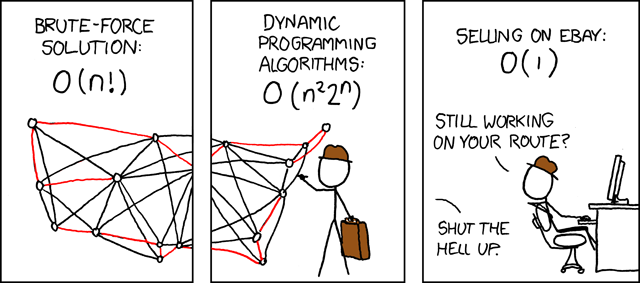
\includegraphics[scale=0.5]{xkcd/tsp_399}
		\caption{ \texttt{\url{http://www.xkcd.com/399}} }
	\end{figure} 	
	}
	

\end{frame}

%\subsection{Warshall-Algorithmus}
%\begin{frame}
%	\only<1>{Schneller geht es mit dem Warshall-Algorithmus!}
%	\only<2>{\begin{align*}
%		&\mathbf{for}\ i\leftarrow 0 \ \mathbf{to} \ n-1 \ \mathbf{do}  \\
%		&\hspace*{2em} \mathbf{for}\ j \leftarrow 0 \ \mathbf{to} \ n-1 \ \mathbf{do} \\
%		& \hspace*{4em} W_{ij} \leftarrow \begin{cases} 1 & i = j \\ A_{ij} & i\neq j \end{cases}  \\
%		&\hspace*{2em} \mathbf{od} \\
%		& \mathbf{od} \\
%		& \mathbf{for}\ k \leftarrow 0 \ \mathbf{to} \ n-1\ \mathbf{do} \\
%		& \hspace*{2em} \mathbf{for}\ i\leftarrow 0 \ \mathbf{to} \ n-1 \ \mathbf{do} \\
%		& \hspace*{4em} \mathbf{for}\ j\leftarrow 0 \ \mathbf{to}\ n-1 \ \mathbf{do} \\
%		& \hspace*{6em} W_{ij} \leftarrow \max\left( W_{ij} , \min(W_{ik},W_{kj}) \right) \\
%		& \hspace*{4em} \mathbf{od}\\
%		& \hspace*{2em} \mathbf{od} \\
%		& \mathbf{od} 	
%		\end{align*}}
%	\only<3>{\begin{align*}
%		&\mathbf{for}\ i\leftarrow 0 \ \mathbf{to} \ n-1 \ \mathbf{do} & // n  \\
%		&\hspace*{2em} \mathbf{for}\ j \leftarrow 0 \ \mathbf{to} \ n-1 \ \mathbf{do} & // n \\
%		& \hspace*{4em} W_{ij} \leftarrow \begin{cases} 1 & i = j \\ A_{ij} & i\neq j \end{cases} & // 1 \\
%		&\hspace*{2em} \mathbf{od} \\
%		& \mathbf{od} \\
%		& \mathbf{for}\ k \leftarrow 0 \ \mathbf{to} \ n-1\ \mathbf{do} & // n \\
%		& \hspace*{2em} \mathbf{for}\ i\leftarrow 0 \ \mathbf{to} \ n-1 \ \mathbf{do} & // n \\
%		& \hspace*{4em} \mathbf{for}\ j\leftarrow 0 \ \mathbf{to}\ n-1 \ \mathbf{do} & // n \\
%		& \hspace*{6em} W_{ij} \leftarrow \max\left( W_{ij} , \min(W_{ik},W_{kj}) \right) & // 1 \\
%		& \hspace*{4em} \mathbf{od}\\
%		& \hspace*{2em} \mathbf{od} \\
%		& \mathbf{od} 	
%		\end{align*}}
%\end{frame}
%
%\begin{frame}
%	\frametitle{Der Warshall-Algorithmus}
%	Da wir hier binäre Werte haben, gilt: $$ \max\left( W_{ij} , \min(W_{ik},W_{kj}) \right) = W_{ij} \vee \left( W_{ik} \wedge W_{kj} \right) $$ \pause 
%	Es ergibt sich insgesamt also eine Laufzeit von $$ n^3+n^2$$ 
%\end{frame}
%
%\begin{frame}
%	\frametitle{Der Warshall-Algorithmus}
%	Was sagt die Matrix $W$ an der Stelle $W_{ij}$ nach dem $k-ten$ Durchlauf im Warshall-Algorithmus aus? \\ \pause
%	Stimmt dieser Algorithmus eigentlich?
%\end{frame}
%
%\begin{frame}
%	\frametitle{Warshall beweisen}
%	\begin{block}{Schleifeninvariante}
%		Für alle $i,j\in \G_n \wedge i\neq j$ gilt : Nach $k$ Durchläufen hat die Matrix den Wert $1$ an der Stelle ($i,j$), genau dann wenn es einen wiederholungsfreien Pfad von $i$ nach $j$ über Knoten in $\G_k$ gibt. Bei $i=j$ steht dort eine $1$. \\
%	\end{block}	
%	
%	\pause
%	Beweis auf Seite 117 im GBI-Skript von Herr Worsch. 
%\end{frame}


%\subsection{Aufgabe 2}
%\begin{frame}
%	\frametitle{Aufgabe 2}
%	Gegeben sei folgende Adjazenzmatrix $$ A = \begin{pmatrix}
%	0 & 1 & 0 & 1 & 1 \\ 0 & 1 & 0 & 1 & 0 \\ 1 & 1 & 0 & 1 & 1 \\ 1 & 1 & 1 & 0 & 1 \\ 0 & 0 & 0 & 0 & 0 
%	\end{pmatrix} $$ 
%	Zeichnen Sie den dazugehörigen Graphen und geben Sie die Initialisierungsmatrix sowie alle Zwischenmatrizen beim Warshall-Algorithmus an. 
%\end{frame}
%
%\subsection{Lösung zu Aufgabe 2}
%\begin{frame}
%	\begin{figure}[H]
%		\begin{tikzpicture}[->,>=stealth,baseline=-5mm]
%		\matrix[matrix of math nodes,nodes={draw,circle,minimum size=9mm,inner sep=2pt},row sep=10mm,column sep=10mm,ampersand replacement=\&]
%		{
%			|(0)| 0 \& \& |(1)| 1 \\
%			\& |(3)| 3 \\
%			|(2)| 2 \& \& |(4)| 4 \\
%		};
%		\draw (0) -- (1);
%		\draw (0) to [bend right] (3);
%		\draw (0) to [bend right] (4) ;
%		\path (1) edge [loop right] ();
%		\draw (1) to [bend right] (3);
%		\draw (2) -- (0);
%		\draw (2) to [bend left] (1);
%		\draw (2) -- (4);
%		\draw (3) to [bend right] (0);
%		\draw (3) to [bend right] (1);
%		\draw (3) -- (2);
%		\draw (3) -- (4);
%		\end{tikzpicture}
%	\end{figure}
%\end{frame}
%
%\begin{frame}
%	$$ W_I = \begin{pmatrix}
%	1 & 1&0&1&1\\0&1&0&1&0\\1&1&1&1&1\\1 & 1 & 1 &1 &1 \\ 0 & 0 & 0 & 0 & 1 
%	\end{pmatrix} $$ \pause
%	$$ W_0 = W_I = W_1 = W_2 $$ \pause
%	$$ W_3 = \begin{pmatrix}
%	1 & 1 & 1 & 1 & 1 \\ 1 & 1 & 1 & 1 & 1 \\ 1 & 1 & 1 & 1 & 1 \\ 1 & 1 & 1 & 1 & 1 \\ 0 & 0 & 0 & 0 & 1 
%	\end{pmatrix} $$ \pause
%	$$ W_4 = W_3 = W$$ 
%\end{frame}

% Hier CS50 Binary Search (Telefonbuchszene) zeigen!
% https://www.youtube.com/watch?v=o4SGkB_8fFs&list=PLhQjrBD2T382VRUw5ZpSxQSFrxMOdFObl
% Spulen!!!
% Video ist ganz gut angekommen, braucht also nicht unbedingt ein Telefonbuch...
% Aber wer eines hat, Live wäre das ganze natürlich noch besser...

\section{Quantitative Aspekte}

% TODO: Mehr und bessere Beispiele, generelle Überarbeitung (VL-Folien)

\subsection{Motivation}
\begin{frame}{Laufzeiten}
	Wir interessieren uns für Laufzeiten von Algorithmen.\\
	Aber wie sollen wir die messen?\\ \pause
	Problem: Rechenzeit auf einem Supercomputing-Cluster nicht mit Rechenzeit auf einem IoT-Chip in der Waschmaschine vergleichbar.\\
	
	\bigskip \pause
	Daher: Zählen der \enquote{ausgeführten Operationen} in Abhängigkeit von der Problemgröße $n$.\\
	Meistens interessiert vor allem der Worst-Case.
\end{frame}

\begin{frame}{Abschätzung}
	Genaue Abschätzungen sind oftmals \textit{sehr schwierig}.\\
	Aber oftmals auch \textit{sehr uninteressant}.\\
	Konstante Faktoren z.B. sind durch die ständigen Verbesserungen bei Prozessoren oftmals für die Praxis irrelevant.\\
	
	\bigskip \pause
	Uns interessiert vor allem das Verhalten für \textit{sehr große} Instanzen.
\end{frame}

%% -----------------------------------------------------------------------------

\subsection{Definitionen}
\begin{frame}{Asymptotisches Wachstum}
	\begin{Definition}
		Zwei Funktionen $f,g: \N_0 \to \R_0^+$ wachsen asymptotisch gleich schnell, wenn es zwei Konstanten $c, c' \in \R^+$ gibt, so dass gilt $$\exists n_0 \in \N_0: \ \forall n \geq n_0: \ c \· f(n) \leq g(n) \leq c' \· f(n) $$
		Man schreibt dafür 
		\begin{align*}
			f &\asymp g \\
			\textbf{oder} \quad f(n) &\asymp g(n) \quad \text{{\small (Ja, das ist auch OK!)}}  
			% Hashtag: „n^2“ ist ein Term und keine Funktion etc... Man müsse doch [n \mapsto n^2] schreiben... VL erlaubt ersteres aber auch.
		\end{align*}
	\end{Definition} \pause
	Diese Relation ist eine Äquivalenzrelation!
\end{frame}

\begin{frame}{Landau-Notation I}
	\begin{Definition}
		$\Theta(f)$ ist die Menge aller Funktionen $g$, die asymptotisch genauso schnell wachsen wie $f$, also $$\Theta(f) := \{ g \mid f \asymp g \}$$
	\end{Definition}
	
	\medskip
	\only<1|handout:1>{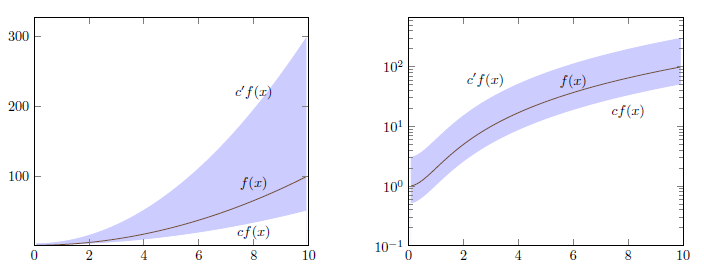
\includegraphics[scale=0.6]{laufzeit/theta1}}
	\only<2|handout:2>{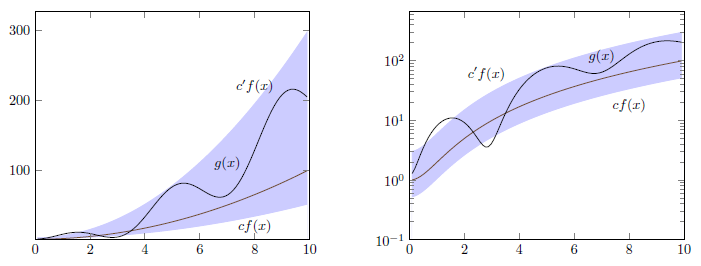
\includegraphics[scale=0.6]{laufzeit/theta2}}
\end{frame}

\begin{frame}{Beispiel}
	$$f(n) := 2 \cdot n^2 + n \qqquad g(n) := n^2$$
	\medskip
	Zeige: $ f \in \Th{g} $.\\ \pause
	Wir suchen $n_0, c, c'$ mit $\forall n \geq n_0: \ c \· g(n) \leq f(n) \leq c' \· g(n) $ \pause
	\medskip
	
	Sei $n \geq 1$, so gilt:\\\pause
	$f(n) = 2 \cdot n^2 + n \leq 2 \cdot n^2 + n^2 = 3 \cdot n^2$ und \\\pause
	$f(n) = 2 \cdot n^2 + n \geq 2 \cdot n^2$
	\medskip
	
	Mit $c := 2$, \, $c' := 3$,\, $n_0 := 1$ ist die Bedingung erfüllt. \qed \pause
	
	\begin{block}{Quiz}
		\TrueQuestion{$n^{100} + 10^9 n^{99} \in \Th{n^{100}}$}
		\FalseQuestion{$2^n \in \Th{n^2}$}
	\end{block}
\end{frame}

\begin{frame}{Beispiel 2}
	\textbf{Behauptung:} \quad $ [n \mapsto \sin(n) + 2] \elem \Th{n \mapsto 1} $ \\ \medskip \pause
	\textbf{Beweis:} \quad Wähle $c := 1, \, c' := 3, \, n_0 := 0$.  \quad Dann gilt $\forall n \geq n_0$: \\
	\begin{align*}
	c \· 1 = 1 &\leq \sin(n) + 2 \leq 3 = c' \· 1 \\
	\text{\Gdw} \qquad  -1 &\leq \sin(n) \leq 1. \qed
	\end{align*}
	\pause
	\Impl Der Sinus ist also „ungefähr“ konstant\only<handout>{ (wenn man seine Brille absetzt \smiley)}.
\end{frame}

\begin{frame}{Asymptotisches Wachstum}
	\begin{Definition}
		Für zwei Funktionen $f,g: \N_0 \to \R_0^+$ definiert man:
		$$g \preceq f \Gdw \exists c \in \R^+ \ \exists n_0 \in \N_0 \ \forall n \geq n_0: \ g(n) \leq c \· f(n)$$
		$$g \succeq f \Gdw \exists c \in \R^+ \ \exists n_0 \in \N_0 \ \forall n \geq n_0: \ g(n) \geq c \· f(n)$$
		(Schreibe analog auch $g(n) \preceq f(n)$ etc.)
	\end{Definition} \pause
	Diese Relationen sind \textbf{keine} Äquivalenzrelationen!
\end{frame}

\begin{frame}[t]{} % erased title due to \includepdf madness... I guess it's not that important anyway. Tags: fake title faketitle include pdf frametitle
	\fakeframetitle{Landau-Notation II}
	\begin{Definition}
		$\Oh{f}$ ist die Menge aller Funktionen $g$, die asymptotisch höchstens so schnell wachsen wie $f$, also $$\Oh{f} := \{ g \mid g \preceq f \}$$
		$\Om{f}$ ist die Menge aller Funktionen $g$, die asymptotisch mindestens so schnell wachsen wie $f$, also $$\Om{f} := \{ g \mid g \succeq f \}$$
	\end{Definition} \pause
	\impl $O$ ist eine Abschätzung nach oben. $\Omega$ ist eine Abschätzung nach unten.
\end{frame}


\setbeamercolor{background canvas}{bg=}

\includepdf[pages=15]{U11.pdf}

\begin{frame}{Eine katastrophale Schreibweise}
	Manchmal (häufig) sieht man auch das, \textbf{NICHT VERWENDEN}:
	$$f = \Theta(g) \qquad h = \Oh{n^3} \qquad k = \Omega(f + g)$$
	\pause
	Dabei ist das $=$ immer als $\in$ zu verstehen!
\end{frame}

\begin{frame}{}
	Ordnet folgende Funktionen nach asymptotischem Wachstum an:
	\begin{itemize}
		\item Identität $f(x) = x$
		\item Konstante Funktion $f(x) = c$
		\item Wurzel
		\item Exponentialfunktion
		\item Logarithmus
	\end{itemize}
\end{frame}

%% Übung: Asymptotische Visualisierungen verschiedener Funktionen
\setbeamercolor{background canvas}{bg=}

\includepdf[pages={5-10}]{U11.pdf}

%\begin{frame}
%	\frametitle{Grenzwertabschätzung}
%	Wir können das auch anders schreiben:
%	\begin{align*}
%	f \in O(g) \qquad &\iff & \qquad 0 \leq  \limsup \limits_{n \to \infty} \frac{f(n)}{g(n)} < \infty \\
%	f \in \Omega(g) \qquad &\iff & \qquad 0 < \liminf  \limits_{n \to \infty} \frac{f(n)}{g(n)} \leq \infty \\
%	f \in \Theta(g) \qquad & \iff & \qquad 0 <  \liminf  \limits_{n \to \infty} \frac{f(n)}{g(n)} \leq  \limsup \limits_{n \to \infty} \frac{f(n)}{g(n)} < \infty
%	\end{align*} \pause
%	Oftmals existiert sogar $\lim$ und wir können $\liminf$ und $\limsup$ vergessen!
%\end{frame}
%
%\begin{frame}{Satz von L'Hospital}
%	\begin{block}{Satz}
%		Gegeben sei $$ \limes{x\to x_0} \frac{f(x)}{g(x)} $$ mit $$ \limes{x\to x_0} f(x) = \limes{x\to x_0} g(x) = 0 \vee \limes{x\to x_0} f(x) = \limes{x\to x_0} g(x) = \infty $$ 
%		Dann gilt 
%		$$ \limes{x\to x_0} \frac{f(x)}{g(x)} = \limes{x\to x_0} \frac{f'(x)}{g'(x)}   $$ mit 
%		$$ f'(x_0) = \left. \frac{\partial f(x)}{\partial x} \right|_{x=x_0} $$ 
%	\end{block}
%\end{frame}
%
%\begin{frame}{Beispiele}
%	Gilt $$ \log n \in \O \left(\sqrt{n}\right) $$ \pause 
%	Betrachte
%	\begin{align*}
%		\limes{n\to\infty} \log n &= \infty \\
%		\limes{n\to\infty} \sqrt{n} &= \infty \\
%		\frac{\partial \log n}{\partial n} &= \frac{1}{n} \\
%		\frac{\partial \sqrt{n}}{\partial n} &= \frac{1}{2} \frac{1}{\sqrt{n}} \\
%		\limes{n\to\infty} \frac{\log n}{\sqrt{n}} &= \limes{n\to\infty} \frac{\frac{1}{n}}{\frac{1}{2} \frac{1}{\sqrt{n}}} \\
%		&= 2 \limes{n\to\infty} \frac{\sqrt{n}}{n}  = 2 \limes{n\to\infty} \frac{1}{\sqrt{n}} = 0 
%	\end{align*}
%\end{frame}

%\subsection{Beispiele}
%\begin{frame}{Polynome}
%	Betrachten wir zwei Polynome $f(n) = n^4 + n^3$ und $g(n) = n^2$: \\
%	Der Quotient $$\frac{f(n)}{g(n)} = \frac{n^4 + n^3}{n^2} = n^2 + n \to \infty$$ Also ist $\lim f/g > 0$ und damit $$g \in O(f) \qquad f \in \Omega(g)$$ aber $\lim f/g = \infty$ also $$f \not \in O(g) \qquad g \not \in \Omega(f)$$ und vor allem $$f \not \in \Theta(g)$$
%\end{frame}

\begin{frame}{Logarithmen}
	\only<handout:0>{Informatiker LIEBEN Logarithmen...\\}
	\begin{block}{Einige Rechenregeln}
		\begin{align*}
			a^{\log_a n} &= n\\
			\log_b n^a &= a \cdot \log_b n\\
			\log_b (n \cdot m) &= \log_b n + \log_b m\\
			a^{\log_b n} &= n^{\log_b a}
		\end{align*}
	\end{block}
\end{frame}

\begin{frame}{Logarithmen}
	\begin{block}{Lemma}
		$$a^{\log_b n} = n^{\log_b a}$$
	\end{block}

	\begin{block}{Herleitung}
		\begin{align*}
			a^{\log_b n} &= \left( b ^{\log_b a} \right) ^{\log_b n}\\
						 &= b^{\log_b a \, \cdot \, \log_b n}\\
						 &= \left( b^{\log_b n} \right) ^{\log_b a}\\
						 &= n^{\log_b a}
		\end{align*}
	\end{block}
\end{frame}

\begin{frame}{Logarithmen: Die Basis ist egal}
	\begin{block}{Lemma}
		$$ \log_a n \in \Th{\log_b n} $$
	\end{block}
	
	\begin{block}{Herleitung}
		Es gilt $$n = a^{\log_a n}$$ \pause
		Daraus ergibt sich: $$ \log_b n = \log_b \left(a^{\log_a n}\right) = \log_a n \; \cdot \log_b a $$ \pause 
		Setze $c = c' = \log_b a$, dann ist $$c \· \log_a n \leq \log_b n \leq c' \· \log_a n.$$
	\end{block}
\end{frame}

\begin{frame}{Rechenregeln (I)}
	Einige Rechenregeln im $O$-Kalkül
	\begin{itemize}[<+->]
		\item Für $a > 0$ ist $a \cdot f \in \Th{f}$ 
		\item Für Konstanten $c, d \geq 0$ gilt: \\ 
			\quad $f(n) \in \Oh{g(n)} \Impl f(n) + c \in \Oh{g(n) + d}$ \\
			\quad $f(n) \in \Om{g(n)} \Impl f(n) + c \in \Om{g(n) + d}$ \\
		\item Für $0 < a < b$ ist $n^a \preceq n^b$
		\item Für $a,b > 1$ ist $n^a \preceq b^n$ \qquad {\small (Exponentialfktnen. wachsen stärker als Polynome)}
		\item Für Polynome $f,g$ gilt: \\
			\quad $\mathop{\text{grad}} f = \mathop{\text{grad}} g \iff f \asymp g $
		\item Für $a,b > 0$ gilt $\log_a(n) \in \Theta(\log_b n)$
		
	\end{itemize}
\end{frame}


\begin{frame}{Rechenregeln (II)}
	Weitere Rechenregeln im $O$-Kalkül:
	\begin{itemize}[<+->]
		\item $f \in O(g) \iff g \in \Omega(f)$
		\item $\Theta(f) = O(f) \cap \Omega(f)$ und $f \asymp g \iff f \preceq g \wedge f \succeq g$ 
		\item $O(f_1) + O(f_2) = O(f_1 + f_2)$
		\item Wenn $g \in O(f)$, dann ist auch $O(g) \subseteq O(f)$ und $O(f + g) = O(f)$
	\end{itemize}
	
\end{frame}

%\subsection{Laufzeiten Angeben}
%
%\begin{frame}[fragile]
%	\frametitle{Algorithmus}
%		\verb+int x = 1;+ \\
%		\verb/for (int i = 0; i < n; i++) {/ \\
%		\verb+	x = a * x;+ \\
%		\verb+}+ \\
%		\verb+return(x);+ \\[1em]
%		 \pause
%	Was tut der? \pause Welche Laufzeit hat er?
%\end{frame}
%
%\begin{frame}[fragile]
%	\frametitle{Laufzeiten}
%		\verb+int x = 1;+ \\ \pause $O(1)$ \\ \pause
%		\verb/for (int i = 0; i < n; i++) {/ \\  \pause $O(1), O(1)$ \\ \pause
%		\verb+	x = a * x;+ \\  \pause $O(1)$ \\ \pause
%		\verb+}+ \\  \pause $n$-mal \\ \pause
%		\verb+return(x);+ \\  \pause $O(1)$ \\ \pause
%		 \pause
%		$$O(1 + n + n + 1) = O(n)$$
%\end{frame}


\begin{frame}	
	\begin{block}{Was ihr nun wissen solltet}
		\begin{itemize}
			\item Graphen und ihre Darstellungen
			\item Adjazenz- und Wegematrizen und wie man sie (schnell) ausrechnen kann
			\item Lizenz zum Schludern: O-Kalkül
		\end{itemize}
	\end{block}
	
	\begin{block}{Was nächstes Mal kommt}
		\begin{itemize}
			\item Einfache Laufzeitabschätzungen mit dem Master-Theorem
			\item Endliche Automaten: Mealy und Moore
			\item Endliche Akzeptoren
			%TODO nexttut
			%\item Grenzen endlicher Automaten -- Wer kann zählen?
			%\item Ein Regelwerk für einen Ausdruck -- Reguläre Ausdrücke
		\end{itemize}
	\end{block}
\end{frame}


%TODO replacement?
\thasse{\lastframe{0.5}{0}{xkcd/proofs_1724.png}{https://www.xkcd.com/1724/}}
\slideThanks

\end{document}